\begin{figure}[ht]
\begin{subfigure}[b]{0.48\textwidth}
\centering
\tikzsetnextfilename{newton_divergence}
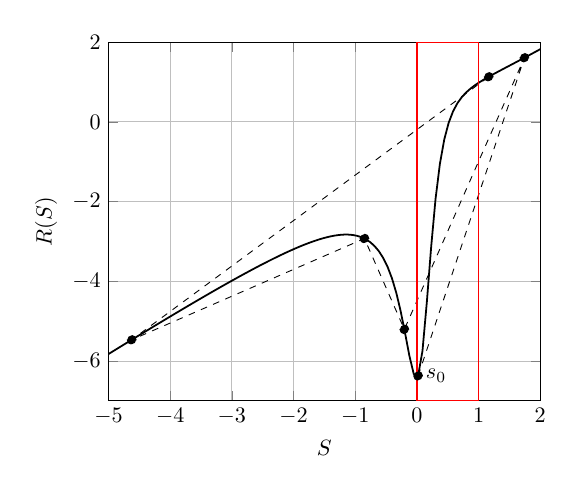
\begin{tikzpicture} [scale=0.8]
	\begin{axis}[
		xlabel={$S$},
		ylabel={$R(S)$},
		xmin = -5,
		xmax = 2,
		ymin = -7,
		ymax = 2,
		domain = -5:2,
		samples = 100,
		grid = major
		]
	\addplot [mark=none, thick] {x - 0.02 + 20000/500*(0.16*x^2/(x^2+0.1*(1-x)^2) - 0.16};
	\addplot[mark=*,style=dashed] coordinates {
		(0.02,-6.373455)
		(1.7437,1.6094)
		(-0.20277,-5.2064)
		(-0.84995,-2.9272)
		(-4.624,-5.4688)
		(1.1646,1.1318)
	};
	\draw [red, thick] (axis cs:0,-7) rectangle (axis cs:1,2);
	\node [right] at (axis cs:0.02,-6.373) {$s_0$};
	\end{axis}
\end{tikzpicture}
\caption{Regular Newton}
\label{fig:newton_divergence}
\end{subfigure}
\begin{subfigure}[b]{0.48\textwidth}
\centering
\tikzsetnextfilename{newton_jtr_convergence}
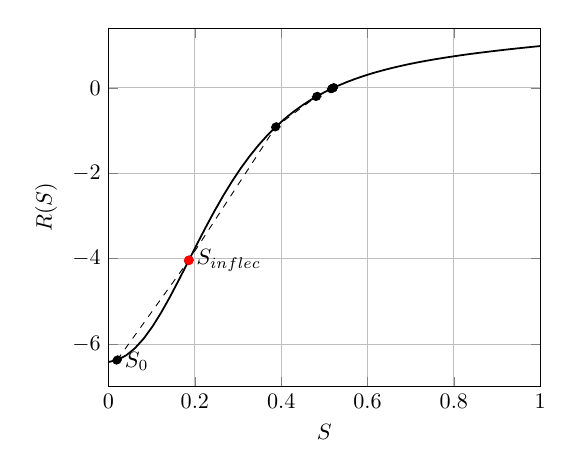
\begin{tikzpicture} [scale=0.8]
	\begin{axis}[
		xlabel={$S$},
		ylabel={$R(S)$},
		xmin = 0,
		xmax = 1,
		ymin = -7,
		ymax = 1.4,
		domain = 0:1,
		samples = 50,
		grid = major,
		clip mode = individual
		]
	\addplot [mark=none, thick] {x - 0.02 + 20000/500*(0.16*x^2/(x^2+0.1*(1-x)^2) - 0.16)};
	\addplot[mark=*,style=dashed] coordinates {
		(0.02,-6.373455)
		(0.18599,-4.0388)
		(0.38741,-0.91277)
		(0.48218,-0.19958)
		(0.51688,-0.017337)
		(0.5205,-0.00016236)
		(0.52053,-1.4564e-08)
	};
	\node [right] at (axis cs:0.02,-6.4) {$S_0$};
	\node [right] at (axis cs:0.18599,-4.0388) {$S_{\text{inflec}}$};
	
	\filldraw [red] (axis cs:0.18599,-4.0388) circle (2pt);
	
	\end{axis}
\end{tikzpicture}
\caption{JTR Newton} \label{fig:newton_jtr_convergence}
\end{subfigure}
\caption{Newton iterations showing the JTR scheme converging unlike the regular Newton updates on the residual in Equation (\ref{eq:residual_two_phase_transport}) with $\Delta t = \unit[20000]{s}$, $\phi_V = 0.5$, $m(V) = \unit[1]{m^3}$, $F_V^- = \unit[0.16]{m^3/s}$, and $Q_V^+ = \unit[-0.16]{m^3/s}$, $\frac{\mu_w}{\mu_o} = 10$, and using initial guess $S_0 = 0.02$. $S_{\text{inflec}}$ is the residual inflection point. The red rectangle marks the range of valid saturations.} \label{fig:newton_methods_viscosity}
\end{figure}